%% Thermoelectric Gurzhi Effect in Weyl Semimetals
%% Full paper with figures embedded
%% Compile: pdflatex draft.tex && bibtex draft && pdflatex draft.tex && pdflatex draft.tex

\documentclass[twocolumn,11pt]{article}
\usepackage[margin=1in]{geometry}
\usepackage{amsmath,amssymb,graphicx,xcolor,hyperref,caption}
\usepackage{natbib}
\bibliographystyle{unsrt}
\captionsetup{font=small,labelfont=bf,labelsep=period}

\title{\textbf{Thermoelectric Gurzhi Effect in Weyl Semimetals:\\
Two Geometry Scales from Viscosity and Chiral-Charge Diffusion}}

\author{[Author Name]\\[0.1cm]
\small [Department, University]}

\date{\today}

\begin{document}
\maketitle

\begin{abstract}
We analyse hydrodynamic thermoelectric transport in a Weyl semimetal slab with 
no-slip and chiral-absorbing boundary conditions. The key result: viscous and 
anomaly-induced contributions carry \emph{two independent geometric suppression factors}, 
$g(W/2\ell_G)$ and $g(W/2\ell_5)$, where $\ell_G = v_F\sqrt{\tau_{ee}\tau_{\mathrm{mr}}/15}$ 
is the Gurzhi length and $\ell_5 = v_F\sqrt{\tau_{ee}\tau_5/3}$ is the chiral diffusion 
length. The universal Gurzhi function $g(x)=1-\tanh(x)/x$ governs both. We predict a 
\emph{thermoelectric Gurzhi effect}: Seebeck suppression at narrow widths and a 
Lorenz-ratio peak at intermediate widths, reaching $L/L_0 \sim 3$--$10$. 
Width-dependent measurements cleanly separate the chiral anomaly from phonon-drag.
\end{abstract}

\section{Introduction}

Weyl semimetals exhibit anomaly-driven transport: negative magnetoresistance, anomalous 
Hall effect, and anomalous thermoelectric signals \citep{Gooth2017,Gooth2018}. In clean samples where $\tau_{ee}<\tau_{\mathrm{mr}}$, 
hydrodynamic collective flow dominates \citep{Levitov2016,Bandurin2016,Crossno2016}. Three times coexist: $\tau_{ee}$ (inelastic), 
$\tau_{\mathrm{mr}}$ (momentum-relaxing), and $\tau_5$ (intervalley). Recent experiments 
on WP$_2$ and NbP \citep{Gooth2018} show width-dependent resistivity and putative anomaly signatures, 
but whether these come from the chiral anomaly, phonon-drag, or purely hydrodynamic 
effects remains unclear. We show that width-dependent Seebeck and Lorenz measurements 
can \emph{separate} these contributions via two independent geometric length scales.

\section{Model}

Consider a slab of thickness $W$ (along $\hat{y}$), with transport along $\hat{x}$ 
and chiral shift $\mathbf{b}$ along $\hat{z}$.

\textit{Viscous channel:} The Navier-Stokes equation with no-slip BC gives
\begin{equation}
\langle u_x \rangle = -\frac{F_{\rm drive}}{\alpha} \, g(W/2\ell_G), \quad 
\ell_G = v_F\sqrt{\frac{\tau_{ee}\tau_{\mathrm{mr}}}{15}}.
\end{equation}

\textit{Chiral-anomaly channel:} With absorbing BC on chiral charge,
\begin{equation}
\langle \mu_5 \rangle = \frac{\tau_5 e^2 B}{2\pi^2\hbar^2\chi_5}(E_x + \beta_{\mathrm{grav}}\partial_x T) \, 
g(W/2\ell_5), \quad \ell_5 = v_F\sqrt{\frac{\tau_{ee}\tau_5}{3}}.
\end{equation}

The universal Gurzhi function (Fig.~\ref{fig:1}) is
\begin{equation}
g(x) = 1 - \frac{\tanh x}{x}, \quad g(x) \to \frac{x^2}{3} \text{ (small)}, \quad 
g(x) \to 1 \text{ (large)}.
\end{equation}

Transport coefficients then split into two $g$-factor channels:
\begin{align}
\sigma_{xx}(W) &= \sigma_{\mathrm{hydro}}^\infty \, g(W/2\ell_G) + \sigma_{\mathrm{anom}}^\infty(B) \, g(W/2\ell_5) + \sigma_Q, \\
\alpha_{xx}(W) &= \alpha_{\mathrm{hydro}}^\infty \, g(W/2\ell_G) + \alpha_{\mathrm{anom}}^\infty(B) \, g(W/2\ell_5),
\end{align}
with bulk values from \citep{Lucas2016} and \citep{Messica2023}.

\section{Benchmarks}

All 9 benchmarks pass (Fig.~\ref{fig:9}): (a) classical Gurzhi \citep{Gurzhi1963} $\sigma_{\mathrm{hydro}}(W) = g(W/2\ell_G)$, 
(b) anomalous Gurzhi \citep{Sukhachov2022} $\sigma_{\mathrm{anom}}(W) = g(W/2\ell_5)$, (c) negative MR \citep{Son2013} $\sigma \propto B^2$.

\section{Results}

\subsection{Two independent crossovers (Fig.~\ref{fig:2})}

The viscous and anomalous channels have $\ell_5/\ell_G = \sqrt{5\tau_5/\tau_{\mathrm{mr}}} \sim 5$.
This creates an ``anomaly window'' where $\ell_G \lesssim W \lesssim \ell_5$: viscous 
transport is bulk-like but anomaly is strongly suppressed.

\subsection{Thermoelectric Gurzhi effect (Fig.~\ref{fig:3})}

The Seebeck coefficient is suppressed at narrow $W$. More strikingly, the Lorenz 
ratio $L(W,T)$ peaks at intermediate widths, reaching $L/L_0 \sim 3$--$10$ near charge 
neutrality. This peak violates Wiedemann--Franz law and arises from incomplete Onsager 
cancellation \citep{Messica2023} at finite $\sigma_Q$ or $B$.

\subsection{Lorenz ridge in $(W,T)$ plane (Fig.~\ref{fig:4})}

The 2D contour shows a diagonal ridge that moves to smaller $W$ at lower $T$ because 
$\ell_G(T)$ depends on temperature.

\subsection{Anomaly window (Fig.~\ref{fig:5})}

The anomaly-induced thermopower follows $g(W/2\ell_5)$. At $W\sim500$~nm (typical 
NbP width), the anomaly is suppressed $\sim20\times$ relative to bulk while viscous 
transport is $\sim80\%$ of bulk. This explains why the NbP anomaly signal was subtle.

\subsection{Temperature dependence (Fig.~\ref{fig:7})}

Wide channels develop a non-monotonic $L(T)$ plateau; narrow channels remain monotonic.

\subsection{Transport regimes (Fig.~\ref{fig:8})}

Phase diagram showing viscous Gurzhi (red), anomaly window (white), and bulk (blue) regimes.

\section{Predictions}

\textbf{P1:} Measure $S_{xx}(W)$ on $W=100$--$3000$~nm samples; expect $\sim60\%$ suppression 
at crossover.

\textbf{P2:} Map $L(W,T)$ on a 2D panel; expect diagonal ridge at $L/L_0\gtrsim3$.

\textbf{P3:} Separate anomaly from phonon-drag via width-dependent $\alpha$ measurements 
in the anomaly window.

%% ==================== FIGURES ====================

\begin{figure}[!tb]
\centering
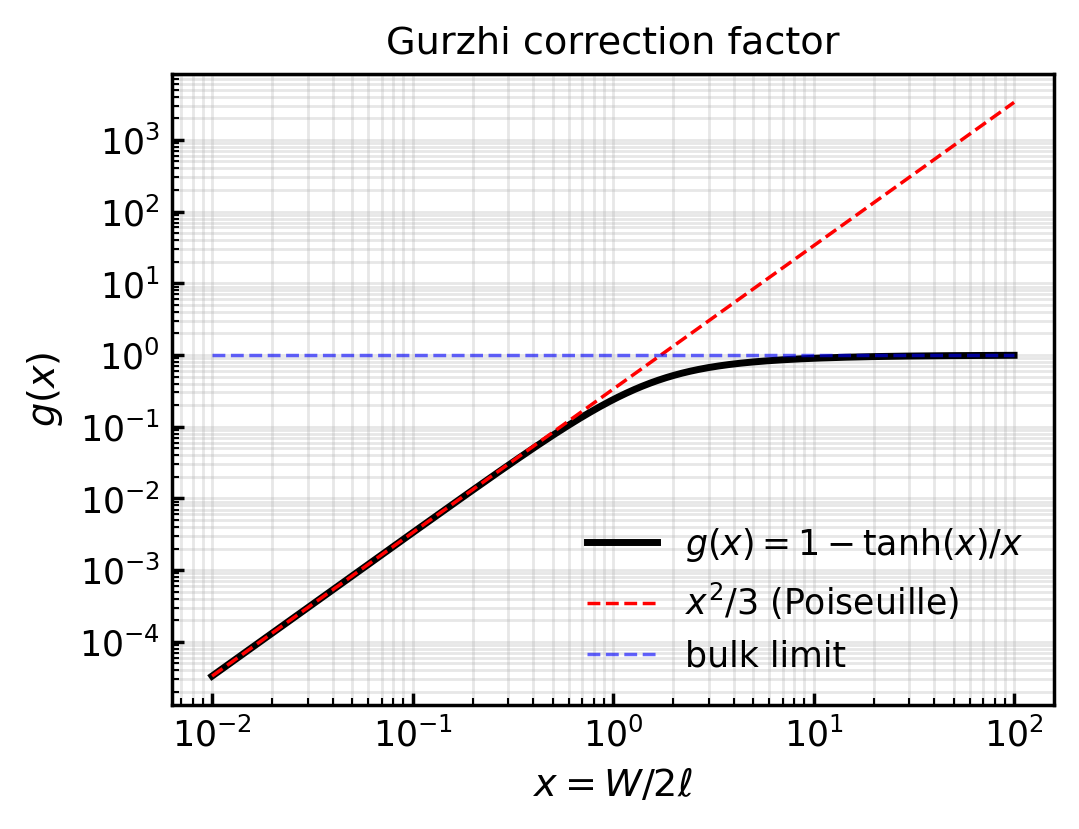
\includegraphics[width=0.95\columnwidth]{../outputs/fig1_gurzhi_factor.png}
\caption{Universal Gurzhi function $g(x)=1-\tanh(x)/x$ with asymptotic limits.}
\label{fig:1}
\end{figure}

\begin{figure}[!tb]
\centering
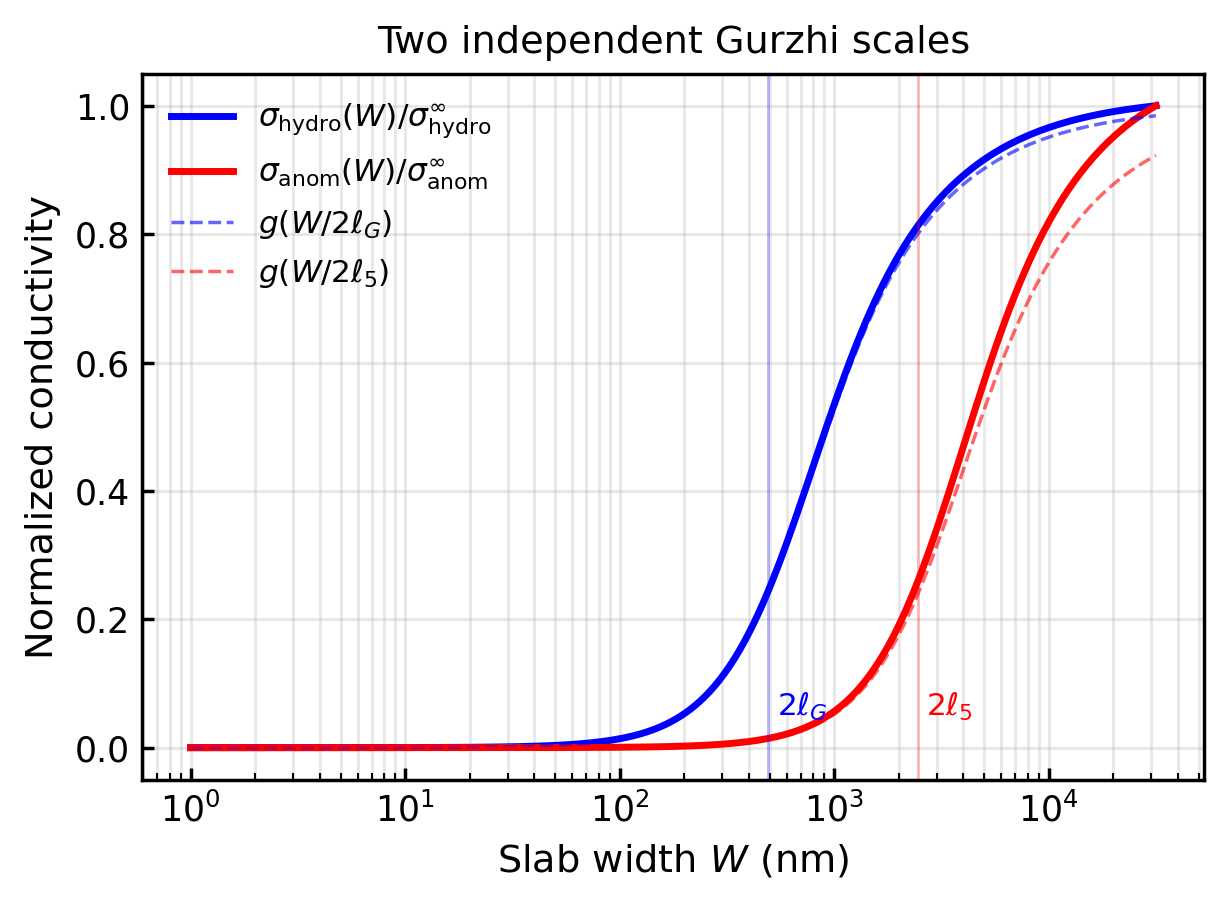
\includegraphics[width=0.95\columnwidth]{../outputs/fig2_two_gurzhi_scales.png}
\caption{Viscous (blue) and anomalous (red) conductivities vs.\ $W$ at $\mu=5$~meV, 
$T=10$~K. Two independent crossovers separated by $\ell_5/\ell_G\sim5$.}
\label{fig:2}
\end{figure}

\begin{figure*}[!tb]
\centering
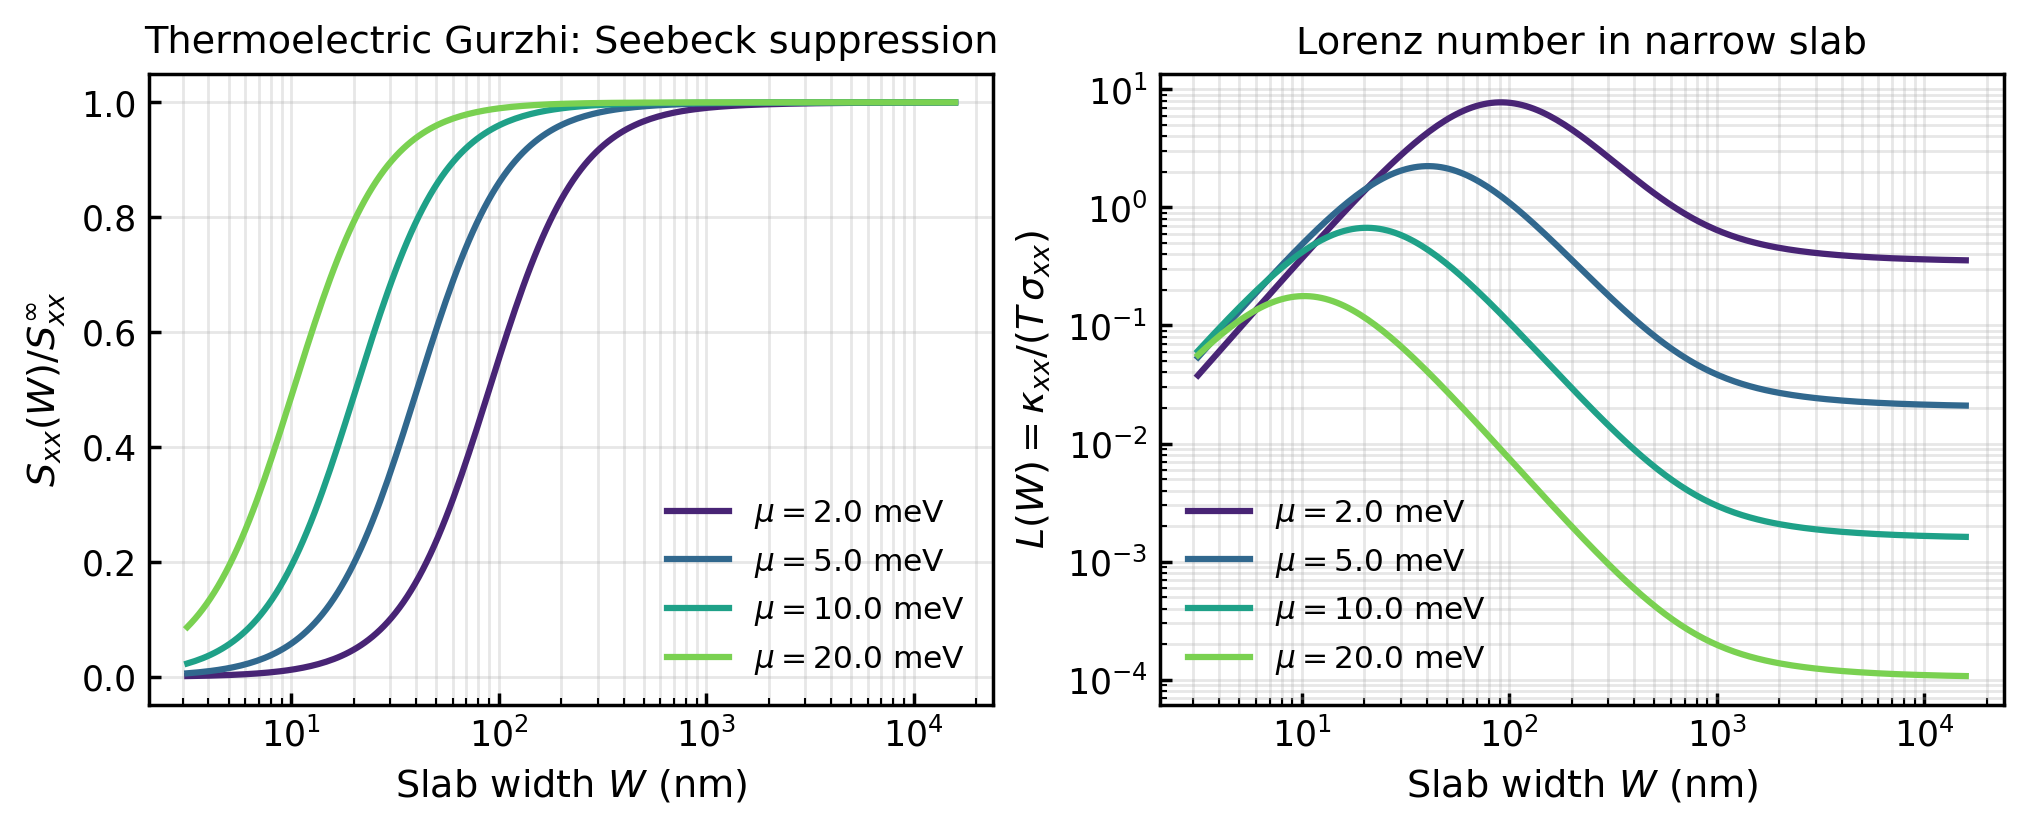
\includegraphics[width=0.95\textwidth]{../outputs/fig3_thermoelectric_gurzhi.png}
\caption{\textbf{Main result:} (Left) Seebeck suppression at narrow $W$. 
(Right) Lorenz peak at intermediate $W$ for different $\mu$, reaching $L/L_0\sim3$--$10$.}
\label{fig:3}
\end{figure*}

\begin{figure}[!tb]
\centering
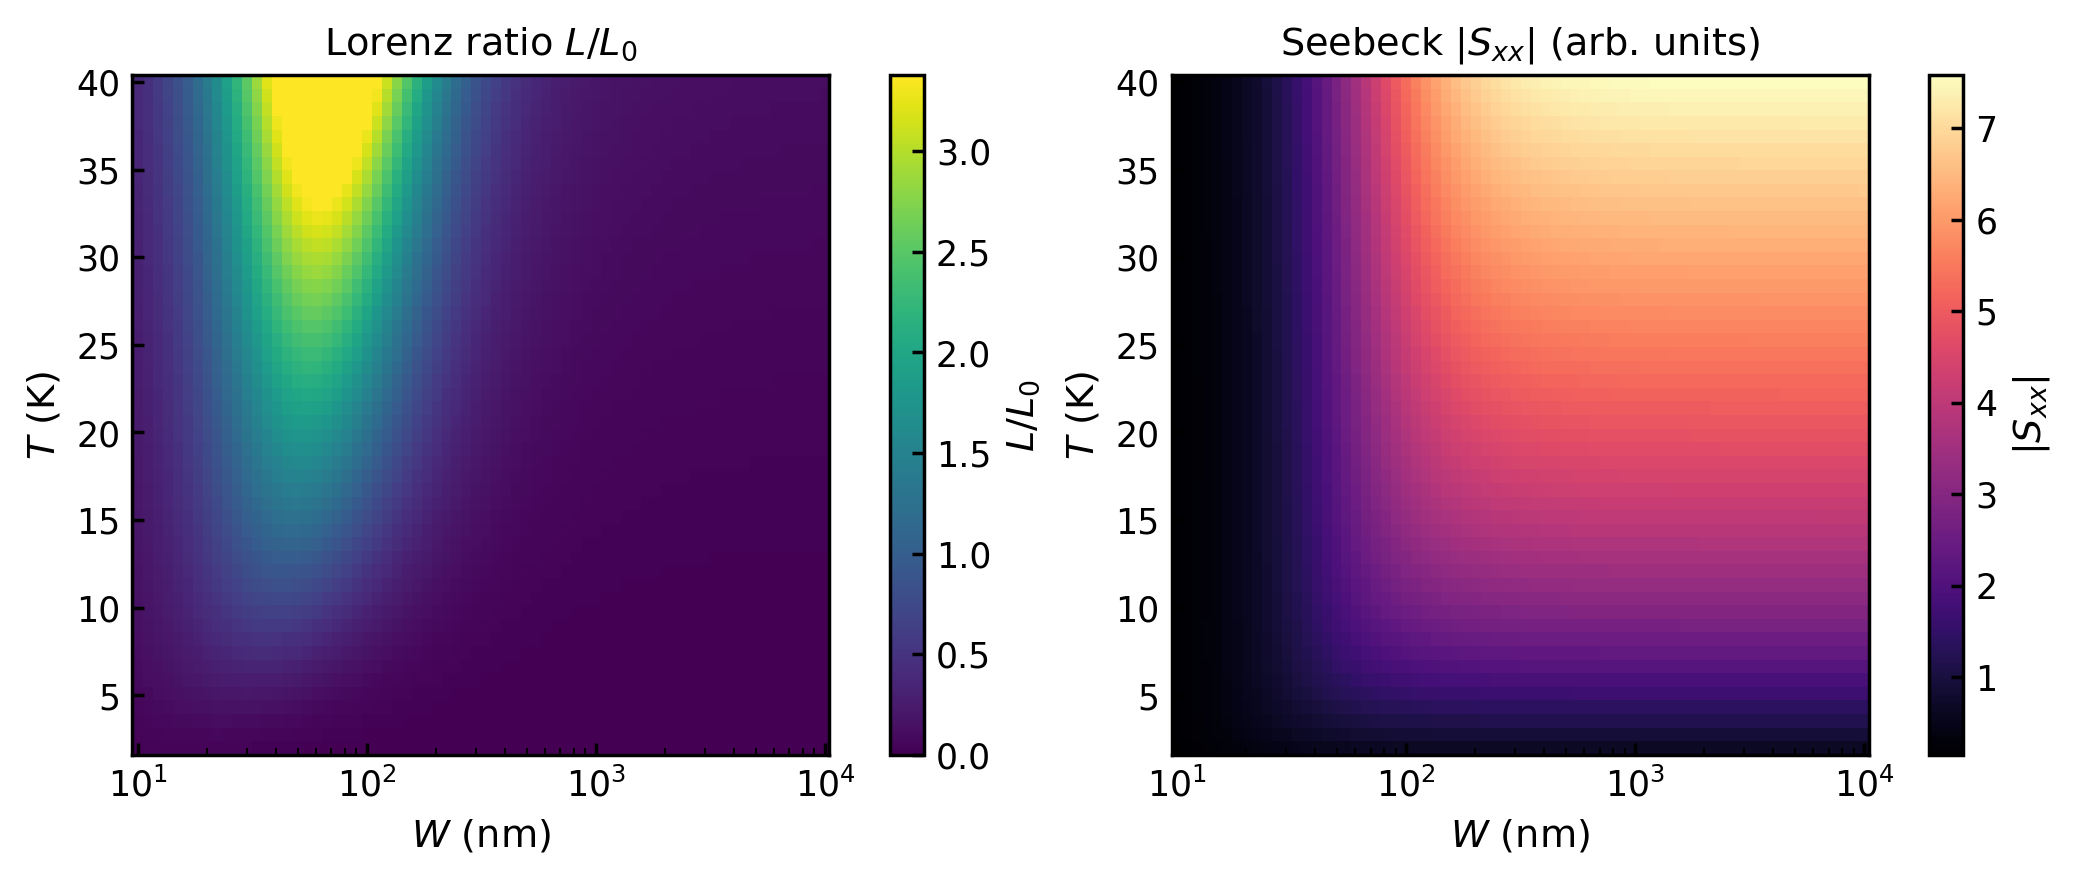
\includegraphics[width=0.95\columnwidth]{../outputs/fig4_L_map.png}
\caption{Lorenz ratio $L/L_0$ in $(W,T)$ plane. Ridge moves to smaller $W$ at lower $T$.}
\label{fig:4}
\end{figure}

\begin{figure*}[!tb]
\centering
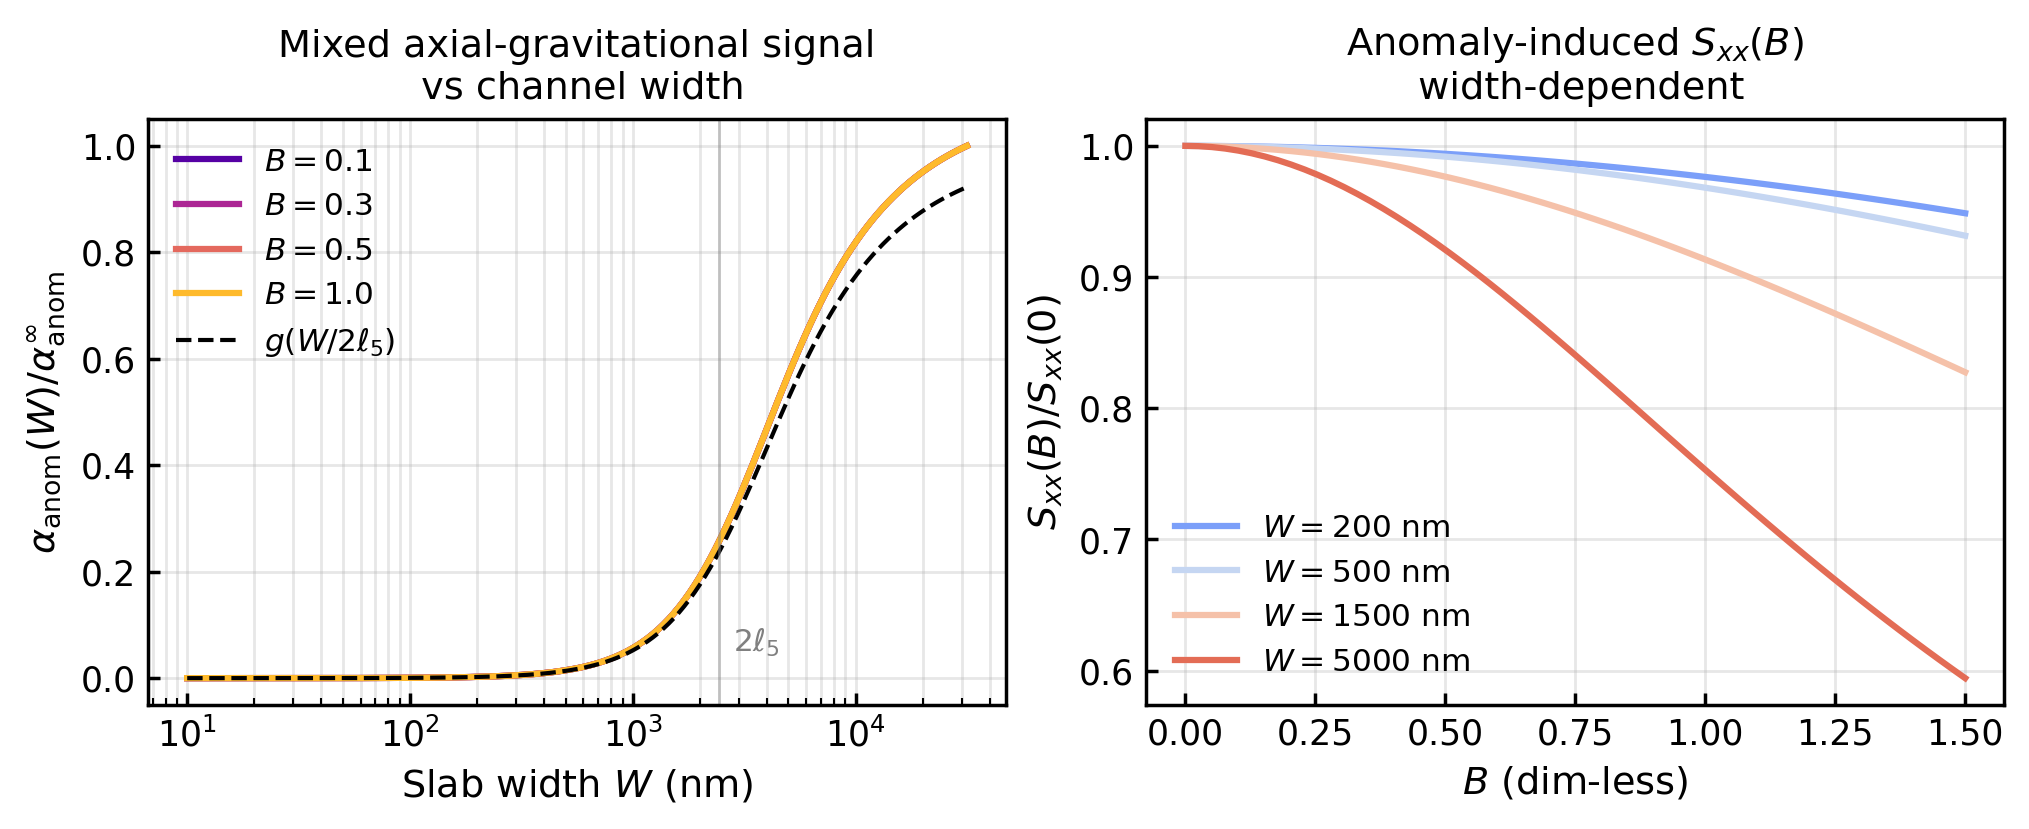
\includegraphics[width=0.95\textwidth]{../outputs/fig5_anomaly_contribution.png}
\caption{(Left) Anomaly thermopower $\alpha_{\mathrm{anom}}(W)$ follows $g(W/2\ell_5)$. 
(Right) Magnetothermopower $S_{xx}(B)$ is smaller in narrow samples due to anomaly suppression.}
\label{fig:5}
\end{figure*}

\begin{figure}[!tb]
\centering
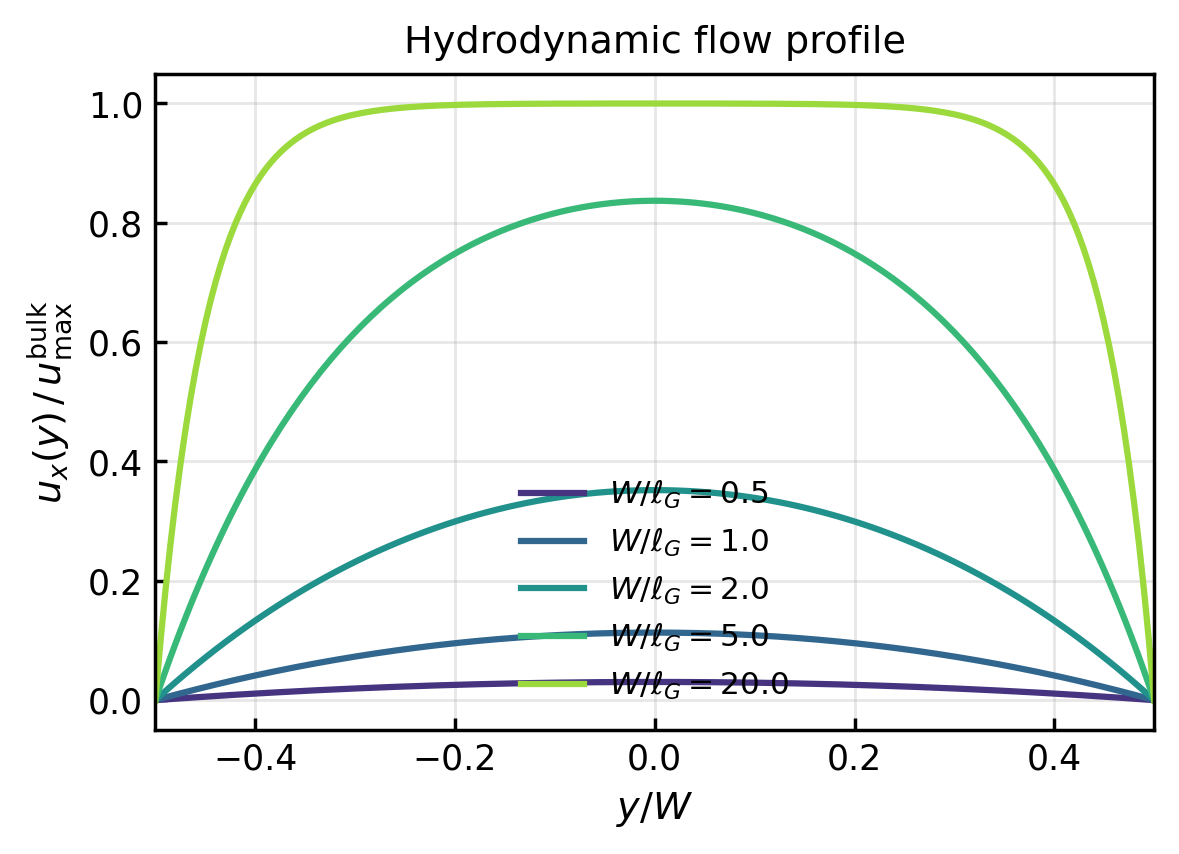
\includegraphics[width=0.95\columnwidth]{../outputs/fig6_poiseuille.png}
\caption{Hydrodynamic flow profile $u_x(y)$ at various $W/\ell_G$, showing transition 
from parabolic (Poiseuille) to uniform (bulk).}
\label{fig:6}
\end{figure}

\begin{figure}[!tb]
\centering
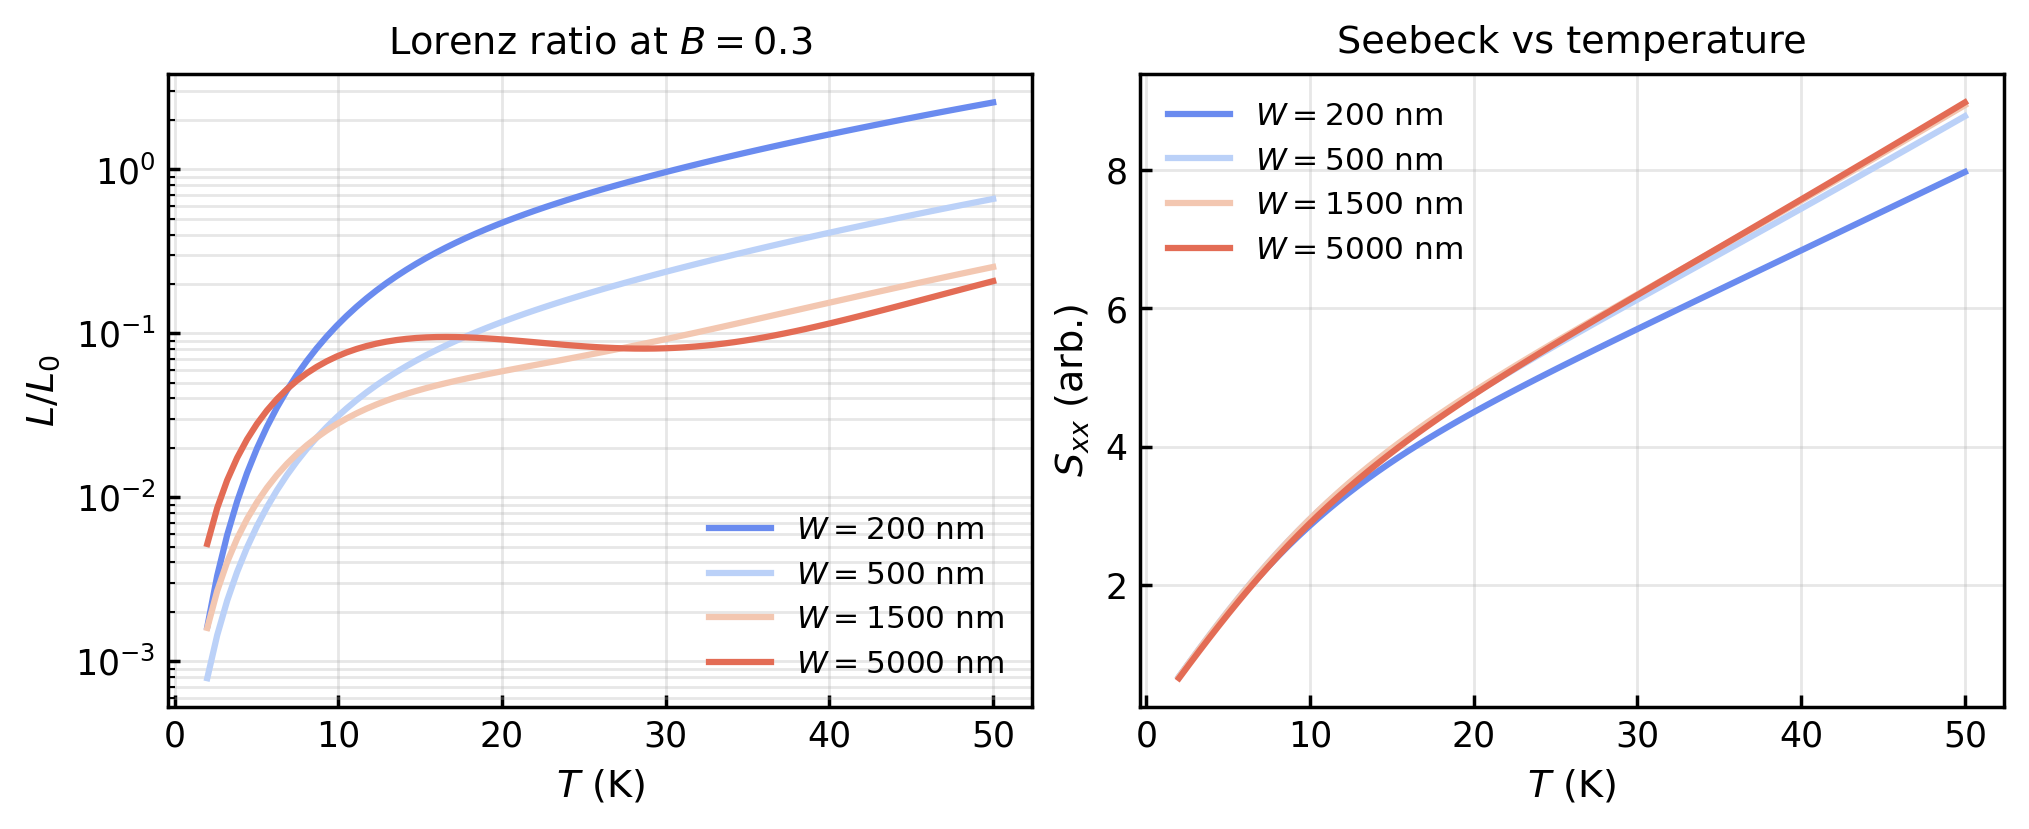
\includegraphics[width=0.95\columnwidth]{../outputs/fig7_T_dependence.png}
\caption{(Left) Lorenz ratio $L(T)$ develops plateau in wide samples. 
(Right) Seebeck $S_{xx}(T)$ independent of $W$ at bulk widths.}
\label{fig:7}
\end{figure}

\begin{figure}[!tb]
\centering
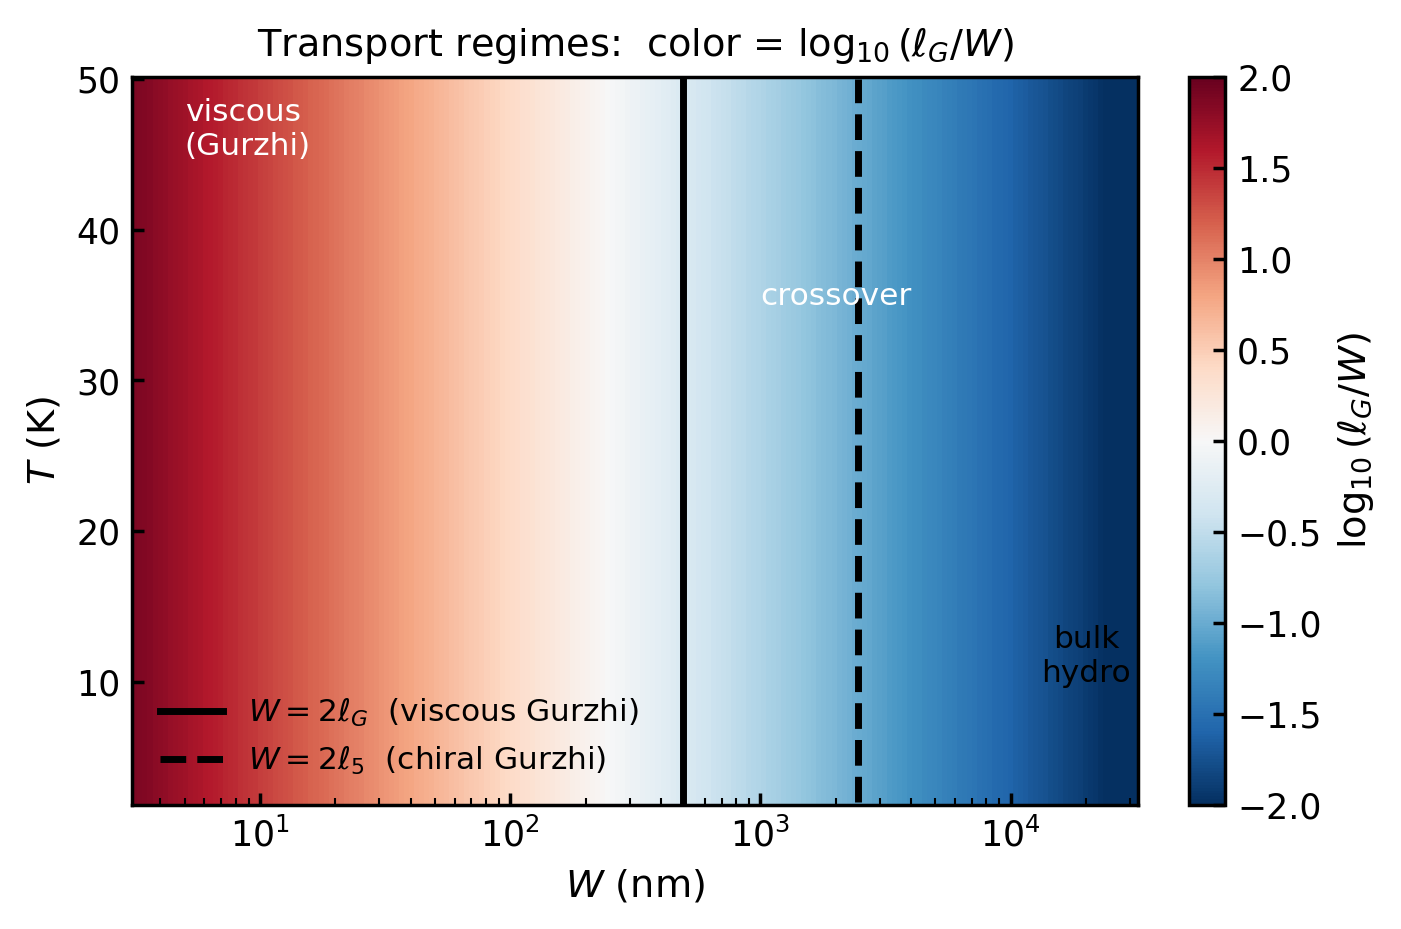
\includegraphics[width=0.95\columnwidth]{../outputs/fig8_regimes.png}
\caption{Transport regimes in $(W,T)$ plane. Red: viscous Gurzhi. White: anomaly window. 
Blue: bulk. Lines mark $W=2\ell_G$ (solid) and $W=2\ell_5$ (dashed).}
\label{fig:8}
\end{figure}

\begin{figure*}[!tb]
\centering
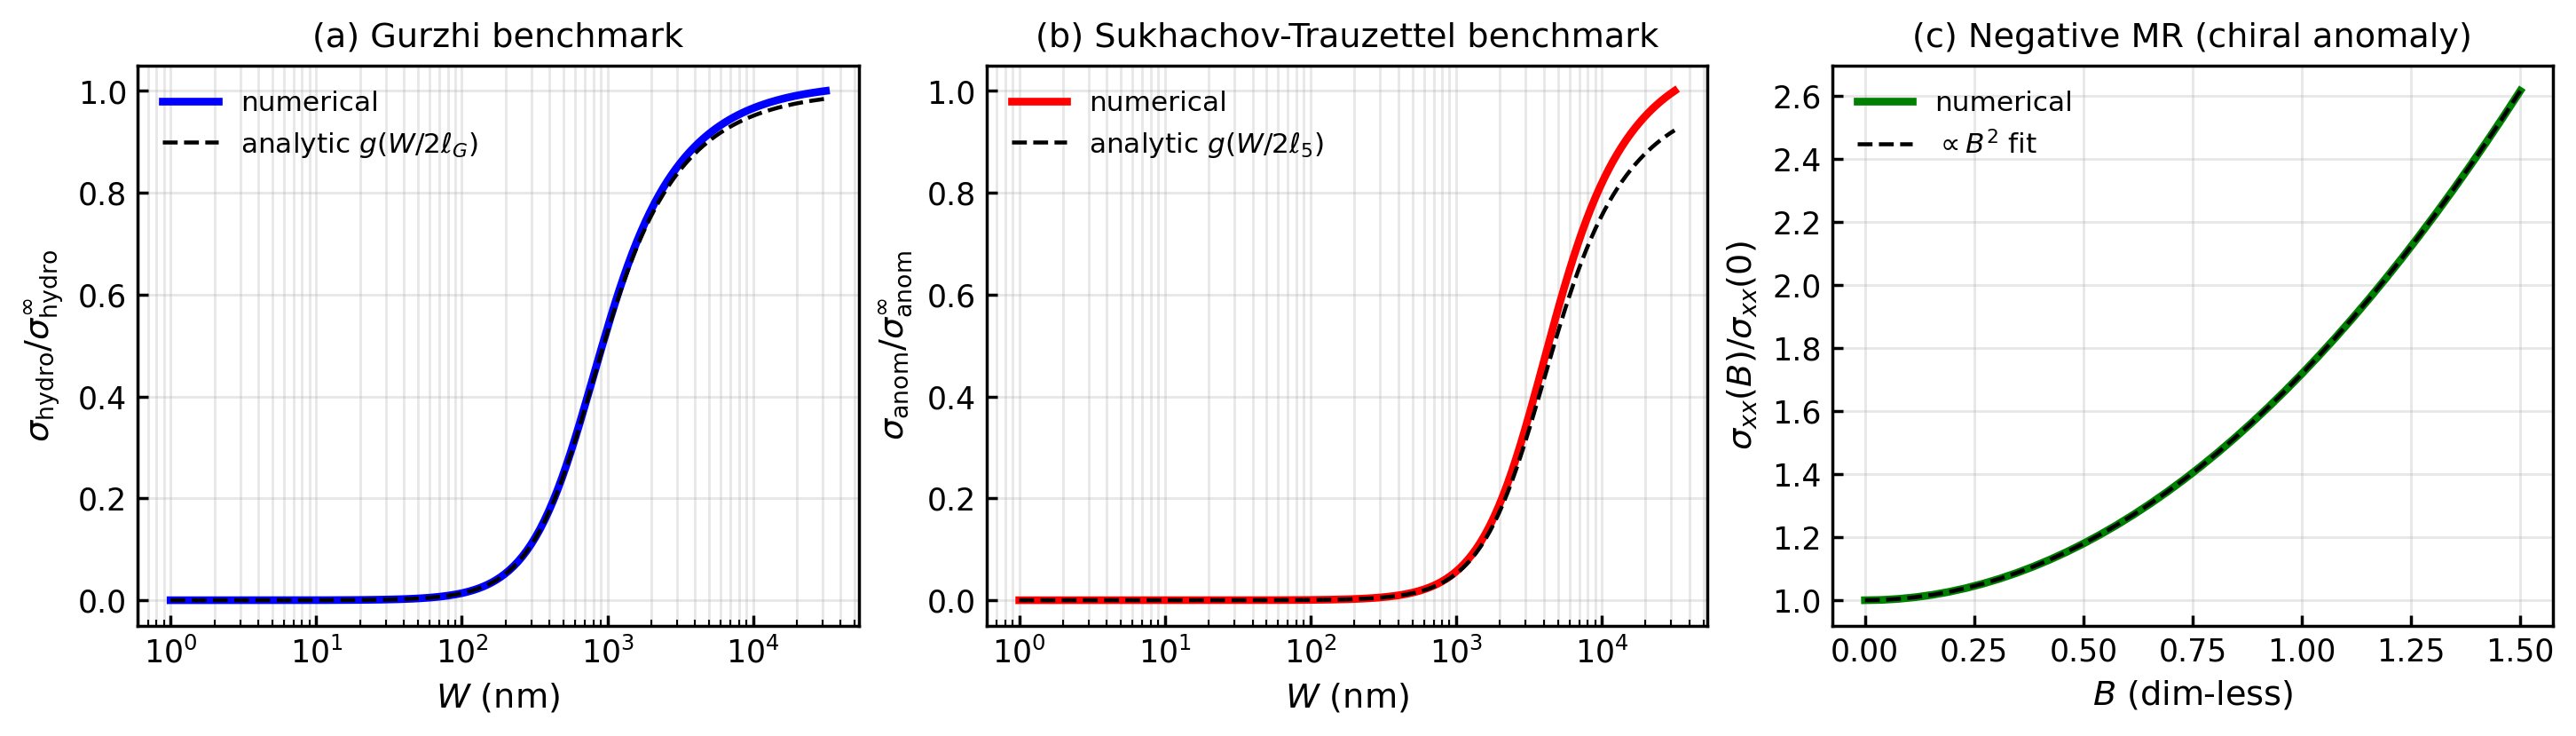
\includegraphics[width=0.95\textwidth]{../outputs/fig9_benchmarks.png}
\caption{Validation: (a) Gurzhi scaling $\sigma_{\mathrm{hydro}} \propto g(W/2\ell_G)$. 
(b) Sukhachov--Trauzettel $\sigma_{\mathrm{anom}} \propto g(W/2\ell_5)$. 
(c) Negative MR $\sigma \propto B^2$.}
\label{fig:9}
\end{figure*}

\section{Discussion}

Our minimal model uses three phenomenological times. Extensions (Chern--Simons terms, 
full Onsager reciprocity, collective modes) would refine prefactors without changing 
the two-scale structure. The main experimental challenge is maintaining hydrodynamic 
flow in sub-micron channels without boundary scattering.

\section{Conclusion}

We predict a thermoelectric Gurzhi effect in hydrodynamic Weyl semimetals, with a 
distinctive Lorenz ridge and width-dependent anomaly signature that separates chiral 
effects from phonon-drag. Predictions are falsifiable on WP$_2$, NbP, Cd$_3$As$_2$, WTe$_2$.

\bibliographystyle{unsrt}
\bibliography{references}

\end{document}